\documentclass[tikz,border=10pt]{standalone}

\begin{document}
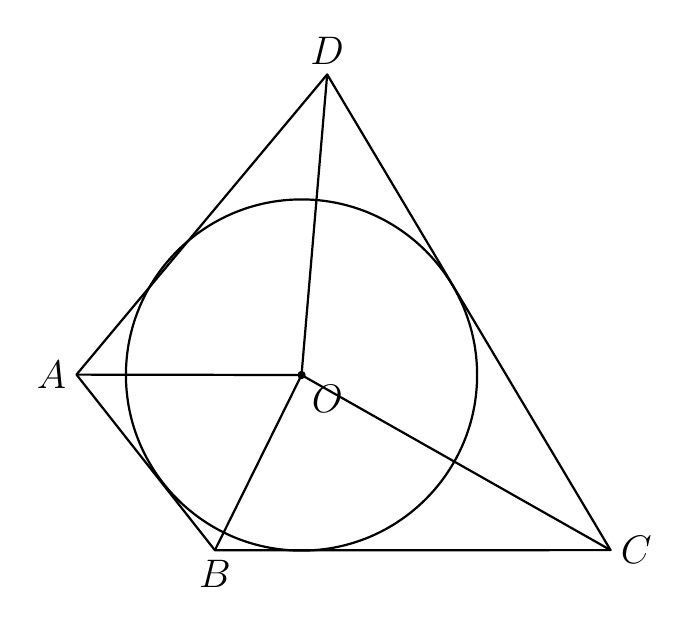
\begin{tikzpicture}[line join=round, line width=0.8pt]
\coordinate (A) at (-3.412,-0.779);
\coordinate (B) at (-1.654,-3.009);
\coordinate (C) at (3.371,-3.008);
\coordinate (D) at (-0.228,3.033);
\coordinate (O) at (-0.554,-0.784);

  
  \draw (A) -- (B) -- (C) -- (D) -- cycle;
  
  \draw (O) -- (A);
  \draw (O) -- (B);
  \draw (O) -- (C);
  \draw (O) -- (D);
  
  \draw (O) circle (2.230);
  
  \fill (O) circle (1.500pt);
  
  \node[left]        at (A) {\fontsize{15.5}{18.6}\selectfont $A$};
  \node[below]       at (B) {\fontsize{15.5}{18.6}\selectfont $B$};
  \node[right]       at (C) {\fontsize{15.5}{18.6}\selectfont $C$};
  \node[above]       at (D) {\fontsize{15.5}{18.6}\selectfont $D$};
  \node[below right] at (O) {\fontsize{15.5}{18.6}\selectfont $O$};
\end{tikzpicture}
\end{document}